\chapter{Data Acquisition}
\label{chapt:DATA_ACQUISITION}
\section{Background}
\subsection{HTML and Xpath}

Internet webpages are written in a markup language called HTML, (HyperText Markup Language). When a webpage is accessed, the html code is sent to the user, and the browser processes and displays the webpage in a human readable format. 

A program written to automatically interpret webpages to extract information, is known as a `scraping' program. The program must process the raw HTML file and access the useful information on the page in an automated fashion. Information is arranged in an html document in a tree-like structure (figure \ref{fig:HTMLTREE}). This example page would display in a browser as a table with 3 rows, each row containing `Table Data A/B/C'. The method of tree traversal is by specifying a path through the document tree on the right, using an `xpath'. 
\begin{figure}[H]
    \centering
    \textbf{HTML and XPaths}\par\medskip
    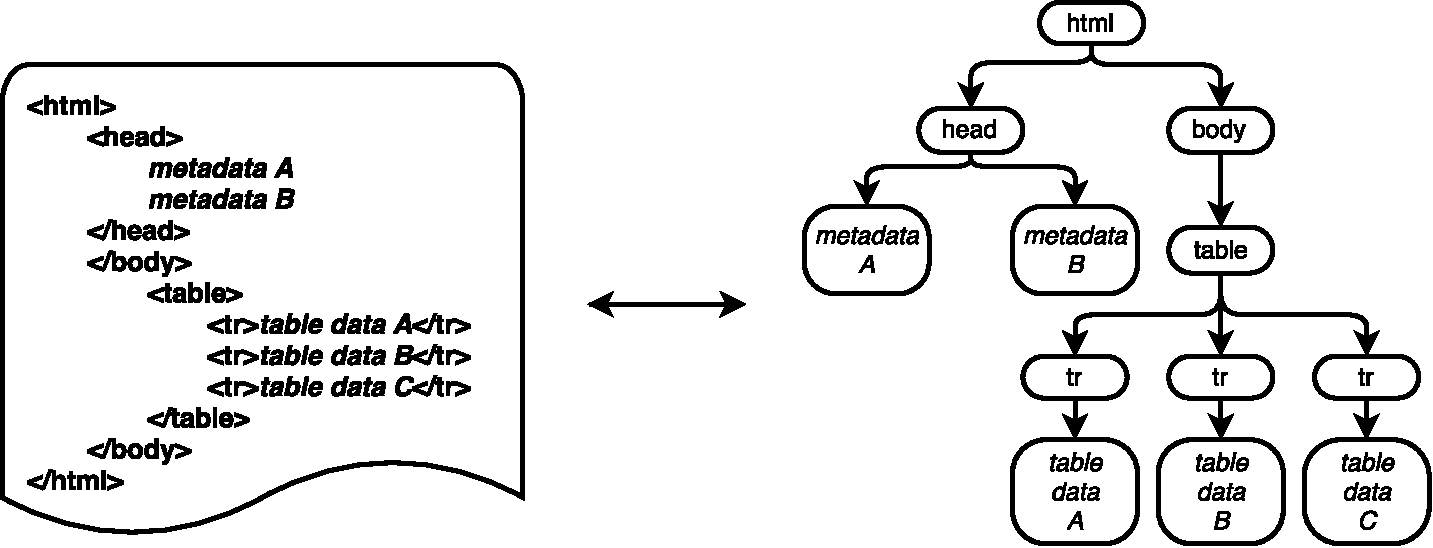
\includegraphics[width=\textwidth]{Data_Acquisition/html_tree.pdf}
    \caption[Tree representation of HTML Code]{Tree representation of HTML code. The html code here displays a table with 3 rows. The page has two peices of metadata associated with it, stored in the `head'.}
        \label{fig:HTMLTREE}

\end{figure}
Xpaths are just paths through the document tree to the desired information. In order the `scrape' the data in the table, the following xpath could be used:
\begin{center}
\texttt{//html/body/tr/*}
\end{center}
This presents an immediate problem, as scraping a millions of webpages requires millions of potentially different xpaths to be known. It is impractical to specify them manually, thus the challenge of large scale scraping is how to identify and collect useful data on webages without manually specifying many xpaths.
\section{Automatic Xpath Generation}
The initial approach was to to analyse the html tree to automatically recognise where useful tabulated or listed data was. The program started at the root of the tree and repeatedly followed the branch with the most `repeating substructure'. The recursive algorithm is summarised below:
\begin{sloppypar}
\begin{enumerate}
\item \texttt{Count \# of descendents of each child node}
\item \begin{enumerate}
\item \texttt{Calculate the pairwise similarities between all child nodes}
\item \texttt{Consider  two nodes similar if pairwise similarity is above a heuristic threshold}
\item \texttt{Calculate proportion of nodes that are considered similar}
\end{enumerate}
\item \texttt{If proportion calculated in (c) is above a heuristic threshold, this node represents a store of information, and the xpath has been found. Otherwise, move to child node with highest \# of descendants, return to step (1)}
\end{enumerate}
\end{sloppypar}
The heuristic thresholds are adjustable parameters. The approach was successful for webpages with large numbers of records, formatted in repeating fashion, but performed poorly for smaller collections of data. As such it was not flexible enough for the task of scraping large for chemical data, and was not implemented in final solution.
\section{Collection Strategy}
As generating xpaths proved unsuitable, a new strategy was required. Chemical information is usually disseminated as journal articles, mostly accompanied by a DOI. By programmatically collecting DOIs, (\S\ref{sec:DOI}) it was possible to build up a large database of chemical information (see  \S\ref{sec:SCRAPING_PROGRAM})
\subsection{DOIS : Document Object Identifiers}
\label{sec:DOI}
DOIs are computer-friendly labels for articles. DOIs are issued by a number of accredited bodies, with the vast majority of chemistry related articles issued by Crossref.\footnote{Crossref is a not-for-profit body comprised from Publishers International Linking Association (PILA), an association of many academic publishers} \cite{crossref-formation}. By pre-pending a DOI string with the url stub \texttt{http://dx.doi.org/}, the International DOI foundation (IDF) service redirects the request to the publisher's website to display the article the DOI refers to. The structure of a DOI is shown in Figure \ref{fig:DOI}.
\begin{figure}[H]
    \centering
    \textbf{Anatomy of a DOI}\par\medskip
    \includegraphics[width=\textwidth]{Data_Acquisition/DOI2.png}
    \caption[Anatomy of a DOI]{Doi structure. The structure consists of a numeric prefix (X and Y must be integers) and alphanumeric suffix (Z can be any Unicode encoded character) \label{fig:DOI}}
\end{figure}
DOIs consist of a prefix and suffix. The prefix is subdivided into the ‘Directory Indicator’ (always integer ‘10’) separated from the ‘Registrant Code’, assigned by the issuing body. Registrant codes are numeric and can be a minimum of 3 integers, with further otpional subdivisions separated by full stops. The suffix is provided by the registrant themselves. It can take any form as long as it is unicode encoded.


It was possible to write a `Regular Expression' pattern matcher (regex) to automatically recognise DOIs within a body of text, (See Figure \ref{fig:REGEX}) The flexibility of the registrant code specification means that DOIs cannot always be unambiguously identified in html documents. 
\begin{figure}[H]
    \centering
    \textbf{Pattern Matching Procedure for DOIs}\par\medskip
    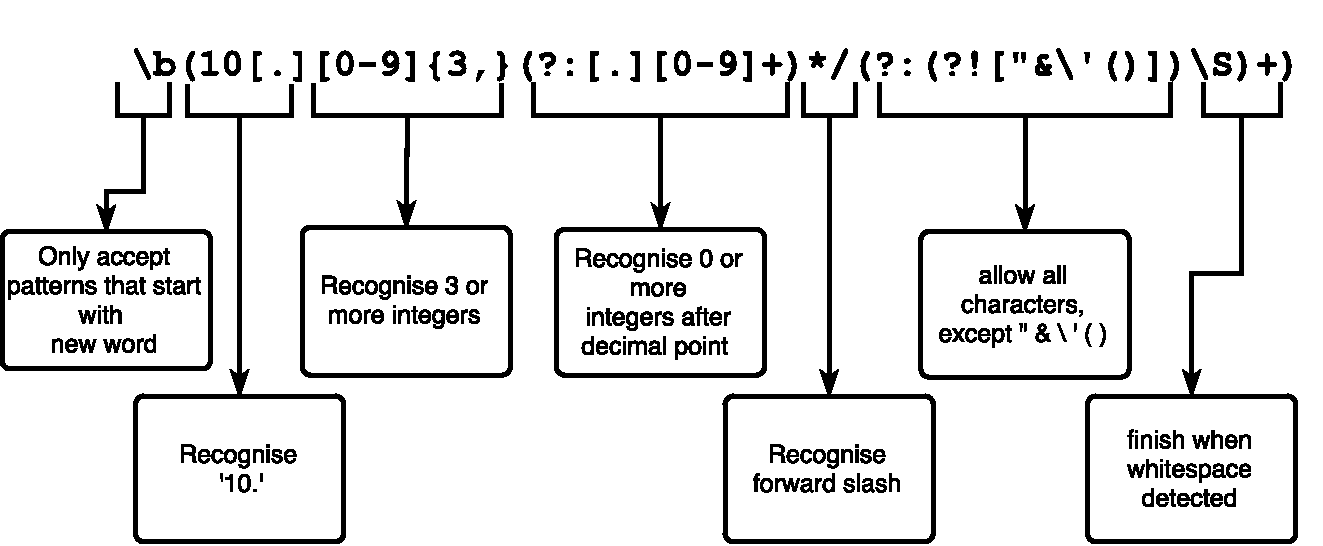
\includegraphics[width=\textwidth]{Data_Acquisition/Regex.pdf}
    \caption[Pattern Matching Procdure for DOIs]{Perl Syntax Regex Code that can identify the vast majority of DOIs within free text) \label{fig:REGEX}}
\end{figure}
Despite this, the regex was able to identify 90.4\% of the dois on the Cambridge University Chemistry Department website \url{http://www.ch.cam.ac.uk/publications}. 
\subsection{Scraping Program}
\label{sec:SCRAPING_PROGRAM}
The Regex approach does not require xpaths in order to extract dois from a webpage. This facilitates large scale scraping from a large set of websites. Some meta-data associated with a DOI can be accessed using an online API exposed by Crossref. Further metadata can be accessed by following the \texttt{http://dx.doi.org/\{DOI\}} redirecting service by DOI $^{\circledR}$ .org. to visit publishers' websites to collect remaining metadata. 

With this methodology in place, a scraping program was written in python to collect DOIs from a list of webpages and collect metadata in a 2 stage process. The Crossref API provides article titles, journals, authors, publisher and publication date meta-data, but not article abstracts. These had to be collected by visiting publisher webpages, and collecting with hand written xpaths. \footnote{Since there are comparatively few publisher websites, only 26 publisher xpaths were required for decent capture coverage.} The procedure is summarised in figure \ref{fig:Cherry} below:
\begin{figure}[H]
    \centering
    \textbf{Scraping Procedure}\par\medskip
    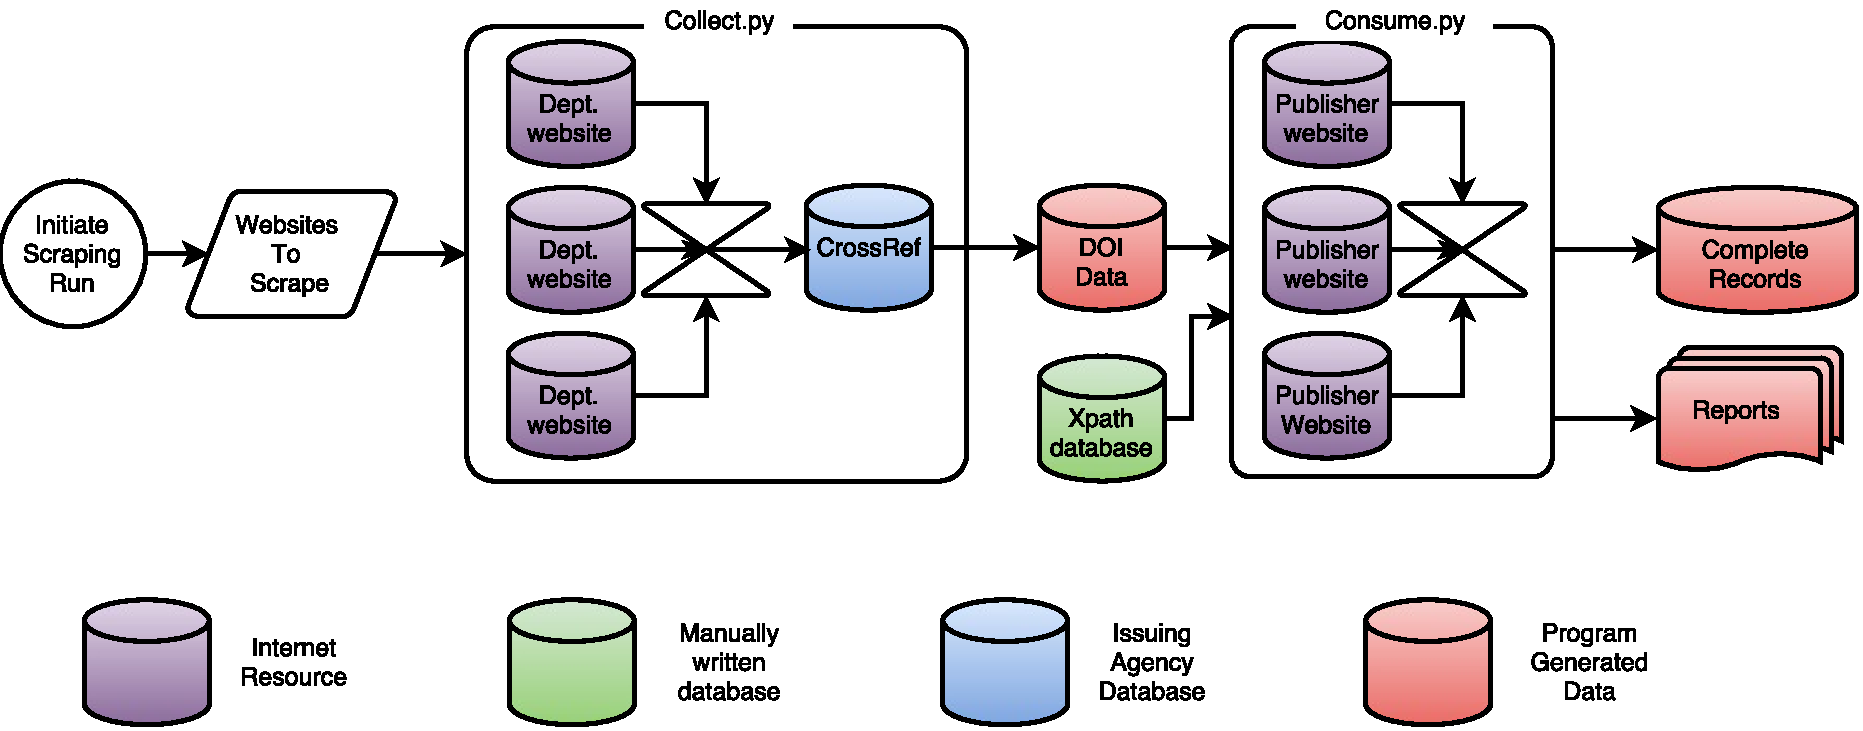
\includegraphics[width=\textwidth]{Data_Acquisition/Cherry2.pdf}
    \caption[Data Flow in Scraping Procedure]{The data flow of the scraping program. Websites from an inputted list of websites are visited and dois are extracted in the process described in  \S\ref{sec:DOI}. The Crossref API service is then used to verify the extracted dois, and collects available meta-data. The program then accesses publisher webpages and collects abstracts. The program also produces explanation of capture failures and some general statistics}
     \label{fig:Cherry}
\end{figure}
The programmatic steps depicted in \ref{fig:Cherry} are:
\begin{sloppypar}
\begin{enumerate}
\item \texttt{Request the webpage from the inputted list}
\item \texttt{Process the html and extract dois}
\item \texttt{Using the Crossref Online API, verify the extracted dois exist.}
\item \texttt{Crossref yields metadata:}
\begin{itemize}
\item \texttt{Title}
\item \texttt{Journal}
\item \texttt{Publisher}
\item \texttt{Authors}
\item \texttt{Publication Date}
\end{itemize}
\item \texttt{for each doi, follow the doi using \texttt{http://dx.doi.org/\{doi\}}}
\item \texttt{use xpath to collect article abstracts.}
\end{enumerate}
\end{sloppypar}
The program exports complete records as .json files, but also feeds directly to a MongoDB database. Once the program was written, the next priority was to obtain a list of webpages to scrape. This is described in  \S\ref{sec:UKSCRAPE} and \S\ref{sec:CROSSREFSCRAPE} 
\section{Collection Results}
\subsection{UK University Department scraping}
\label{sec:UKSCRAPE}
The program was first used to collect the data from the UK. The Goodman group's website hosts a list of UK chemistry departments \url{http://www-jmg.ch.cam.ac.uk/data/c2k/uk.html}. The list was manually checked and some urls were changed to give a list of 68 departments\footnote{Details can be found in the appendix}. The program was run with this list as an input, the results of which are detailed in table \ref{tab:UKSCRAPERES}.
\begin{table}[h!]
\caption{UK Scraping results}
\label{tab:UKSCRAPERES}

\begin{center}
\begin{tabular}{||l|l|l||}
\hline
Process & \# records & \% of maximum yield\\
\hline
Dois collected & 22442 & N/A\%\\
Dois found with metadata & 22397 & 99.8\%\\
Articles successfully resolved & 16363 & 72.9\%\\
Losses due to failed requests & 2753 & 12.3\%\\
Program errors & 133 & 0.6\%\\
Missing Publication Errors & 3148 & 14.0\% \\
\hline
\end{tabular}
\end{center}
\end{table}
Conversion losses were due to 4 components. 45 losses for non-existant dois, 2753 losses to request errors (404 : not-found errors or permission problems), 133 to the program throwing internal errors and 3148 conversions were lost due missing publication xpaths. The 26 specified xpaths \footnote{Corresponding to 37 publishers} were sufficient to convert 83.8\% of successful requests. This was deemed acceptable, as most major publishers had been covered \footnote{see appendix for list of covered publishers}, and the missing publishers each covered a small number of articles it would take another 11 xpaths of the missing most popular publishers to increase the conversion rate from 83.8\% to 90\%.
The efficiency is depicted in figure \ref{fig:UKSANK}

\begin{figure}[H]
    \centering
    \textbf{Efficiency of UK Department Scraping}\par\medskip
    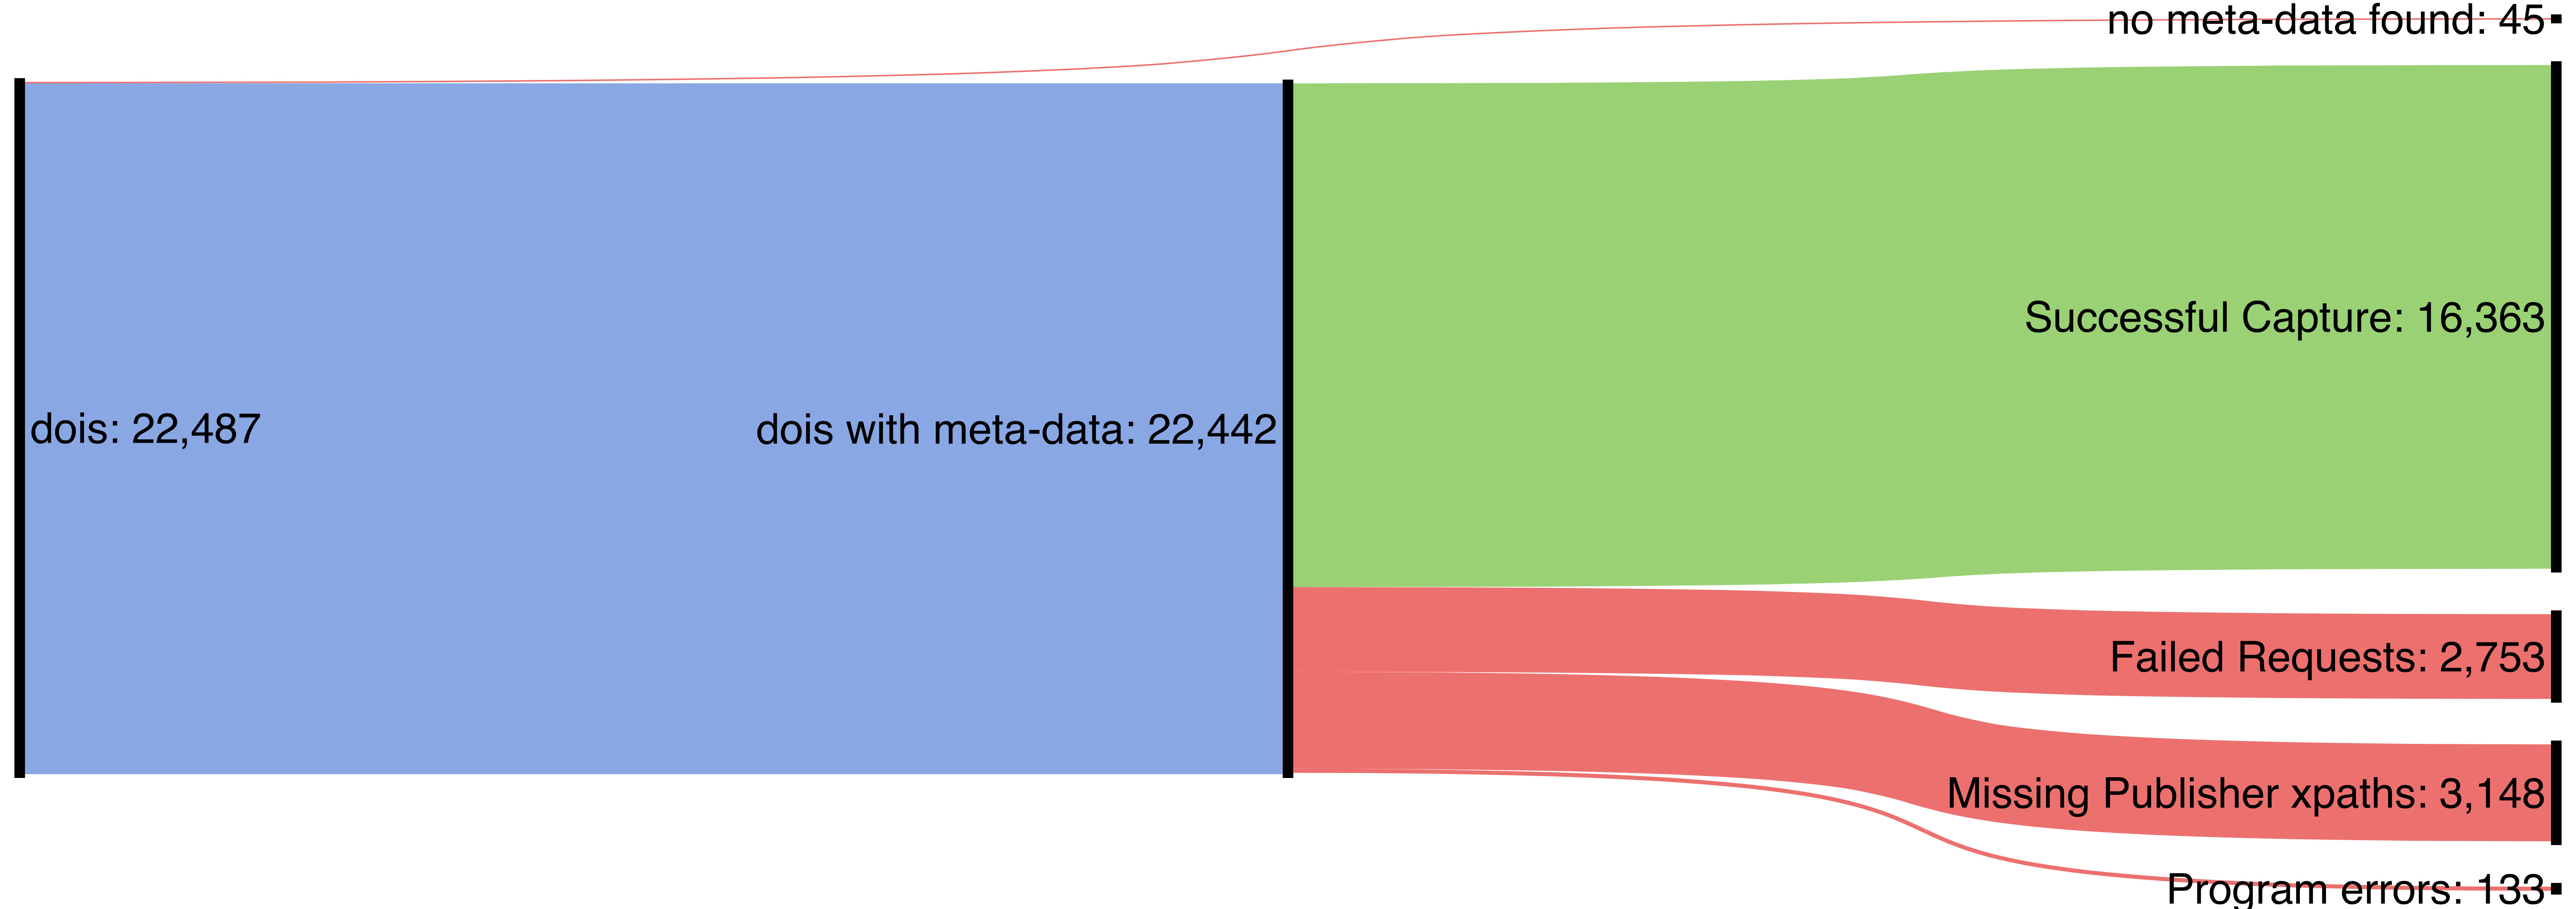
\includegraphics[scale=0.07]{Data_Acquisition/uk_sankey.png}
    \caption[Efficiency of UK Department Scraping]{The loss processes are coloured red, successfully captured full records in green, and the maximum possible yield in blue.}
     \label{fig:UKSANK}
\end{figure}

Interestingly, 9467 out of 16363 successful collections were sourced from \url{http://www.ch.cam.ac.uk}. This could be because the department at Cambridge has an extensive website and also hosts the majority of its information under its own domain name, whereas other departments` data are hosted on central university domains. The scraping program was confined to scrape only webpages belonging directly to chemistry department domains, not the university website as a whole. As a result, it is worth baring in mind that the Cambridge chemistry department may be overrepresented in the UK chemistry data set.

\subsection{Global Scale Scraping}
\label{sec:CROSSREFSCRAPE}
The UK scrape was a respectable start, but much more data would be required to train a machine learning model successfully. One approach would have been expand the scrape to world-wide chemistry departments, and other learn\`{e}d bodies. However, Crossref also exposes a search service that can be used to query its vast internal database. The program was then set up to query the Crossref service for search terms `Chemistry', `Chemical', `Molecule' and Molecular' for journal articles and journal titles. This suggested possible yields in the millions of articles. 

The program was instructed to scrape the search results pages of these queries. Because the scraping job was so large, the program was set up to `pause' before the publisher abstract collection stage.The results of up scrape up to this point were examined before setting off the second stage to collect abstracts.

At the intermediate point, the program had collected 1,267,495 records, which was deemed successful, and would provide enough data to train a powerful machine learning algorithm.

The records were then inspected and publisher distributions were considered. Some of this analysis is presented in \S\ref{sec:SCRAPEANALYSIS}. After careful considerations of request server loads and predicting capture probabilities, the second half of the scraping routine was set off to run for 3 days.
\label{sec:CROSSREFSCRAPE}
\subsection{Problems with ACS and Taylor \& Francis}
Some publishers automatically track request volumes sent to their site as they wish to discourage automatic scraping of their data. Scraping their websites constitutes fair use and is legal in the UK , and despite the university owning a Licence to full access of these publishers' publications, the material collected was freely available without licence\cite{thelaw} \cite{contentminelegal}. However, during the scraping run, a bug in the randomisation of request frequencies resulted in detection by the ACS \footnote{American Chemical Society} and Taylor \& Francis. Both publishers responded by banning the IP address of the computer running the program. The department librarians were able to restore access, and it was agreed that no further large scale scraping runs would be performed. 

Taylor \& Francis banned the IP address after it detected over 100 requests were made within 5 minutes. This corresponds to a request every 3 seconds. This is modest server load compared to other publishers, and was not foreseen to cause problems.

The ACS banning occurred because of a bug in the randomisation of requests. The program was instructed to take a doi from a random publisher every time it made a request, rather than just a random doi. Since the largest publisher was ACS, the program eventually exhausted dois from the other publishers, until there were only ACS dois to `randomly' draw requests from. This meant the request frequency to the ACS server went up dramatically. This uptick broke the threshold of allowed requests at the ACS server which then banned the IP (approximately 10 requests a second).

\begin{figure}[H]
    \centering
    \textbf{ACS BANNING}\par\medskip
    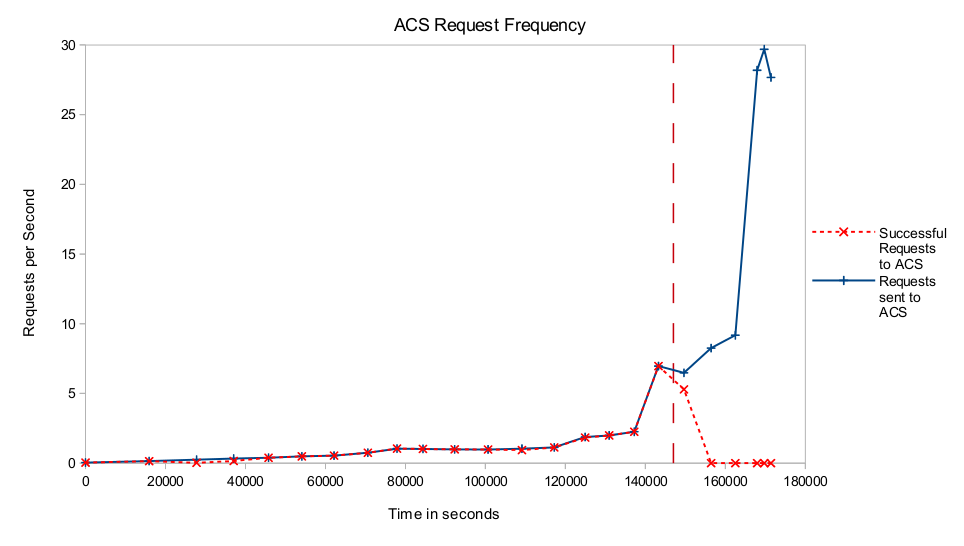
\includegraphics[width=\textwidth]{Data_Acquisition/ACS_crash_line.png}
    \caption[Request Frequency Leading to ACS Ban]{The request frequency is plotted in blue, the received pages frequency in red. The vertical dashed line shows where the server detected the scape and banned the IP.}
     \label{fig:ACSBAN}
\end{figure}
The program was capable of making a total number of approximately 30 requests per seconds. As canbe seen in figure \ref{fig:ACSBAN}, the program began to run out of requests to other publishers after approximately 140,000 seconds, resulting in an increase in the proportion of total requests per second to ACS. The ban occurred after approximately 150,000 seconds, after which there were no more responses received.
\subsection{Analysis of Collected data}
The yield of the global scale scraping run was cut significantly by the ACS banning event. A summary is tabulated in \ref{tab:LARGESCRAPERES}, and shown graphically in figure \ref{fig:LARGESANK}.
\begin{table}[h!]
\caption{Large Scale Scraping Results}
\label{tab:LARGESCRAPERES}

\begin{center}
\begin{tabular}{||l|l|l||}
\hline
Process & \# records & \% of maximum yield\\
\hline
DOIS collected &  1267495 &N/A\\
DOIS collected with meta-data &  1267495 &100.0\%\\

\hline
Predicted maximum capture & 1071506 &  84.5\%\\
Predicted Capture without ACS & 581797 & 45.9\%\\
\hline
Articles successfully captured & 714370 & 56.4\%\\
Losses to failed requests (excluding ACS)& 53743 & 4.2\%\\
Losses to ACS banning & 303393 & 23.9\%\\
Missing Publications \& Program Errors & 195989 & 15.5\%\\
\hline
\end{tabular}
\end{center}
\end{table}
\begin{figure}[H]
    \centering
    \textbf{Efficiency of Large Scale Scraping}\par\medskip
    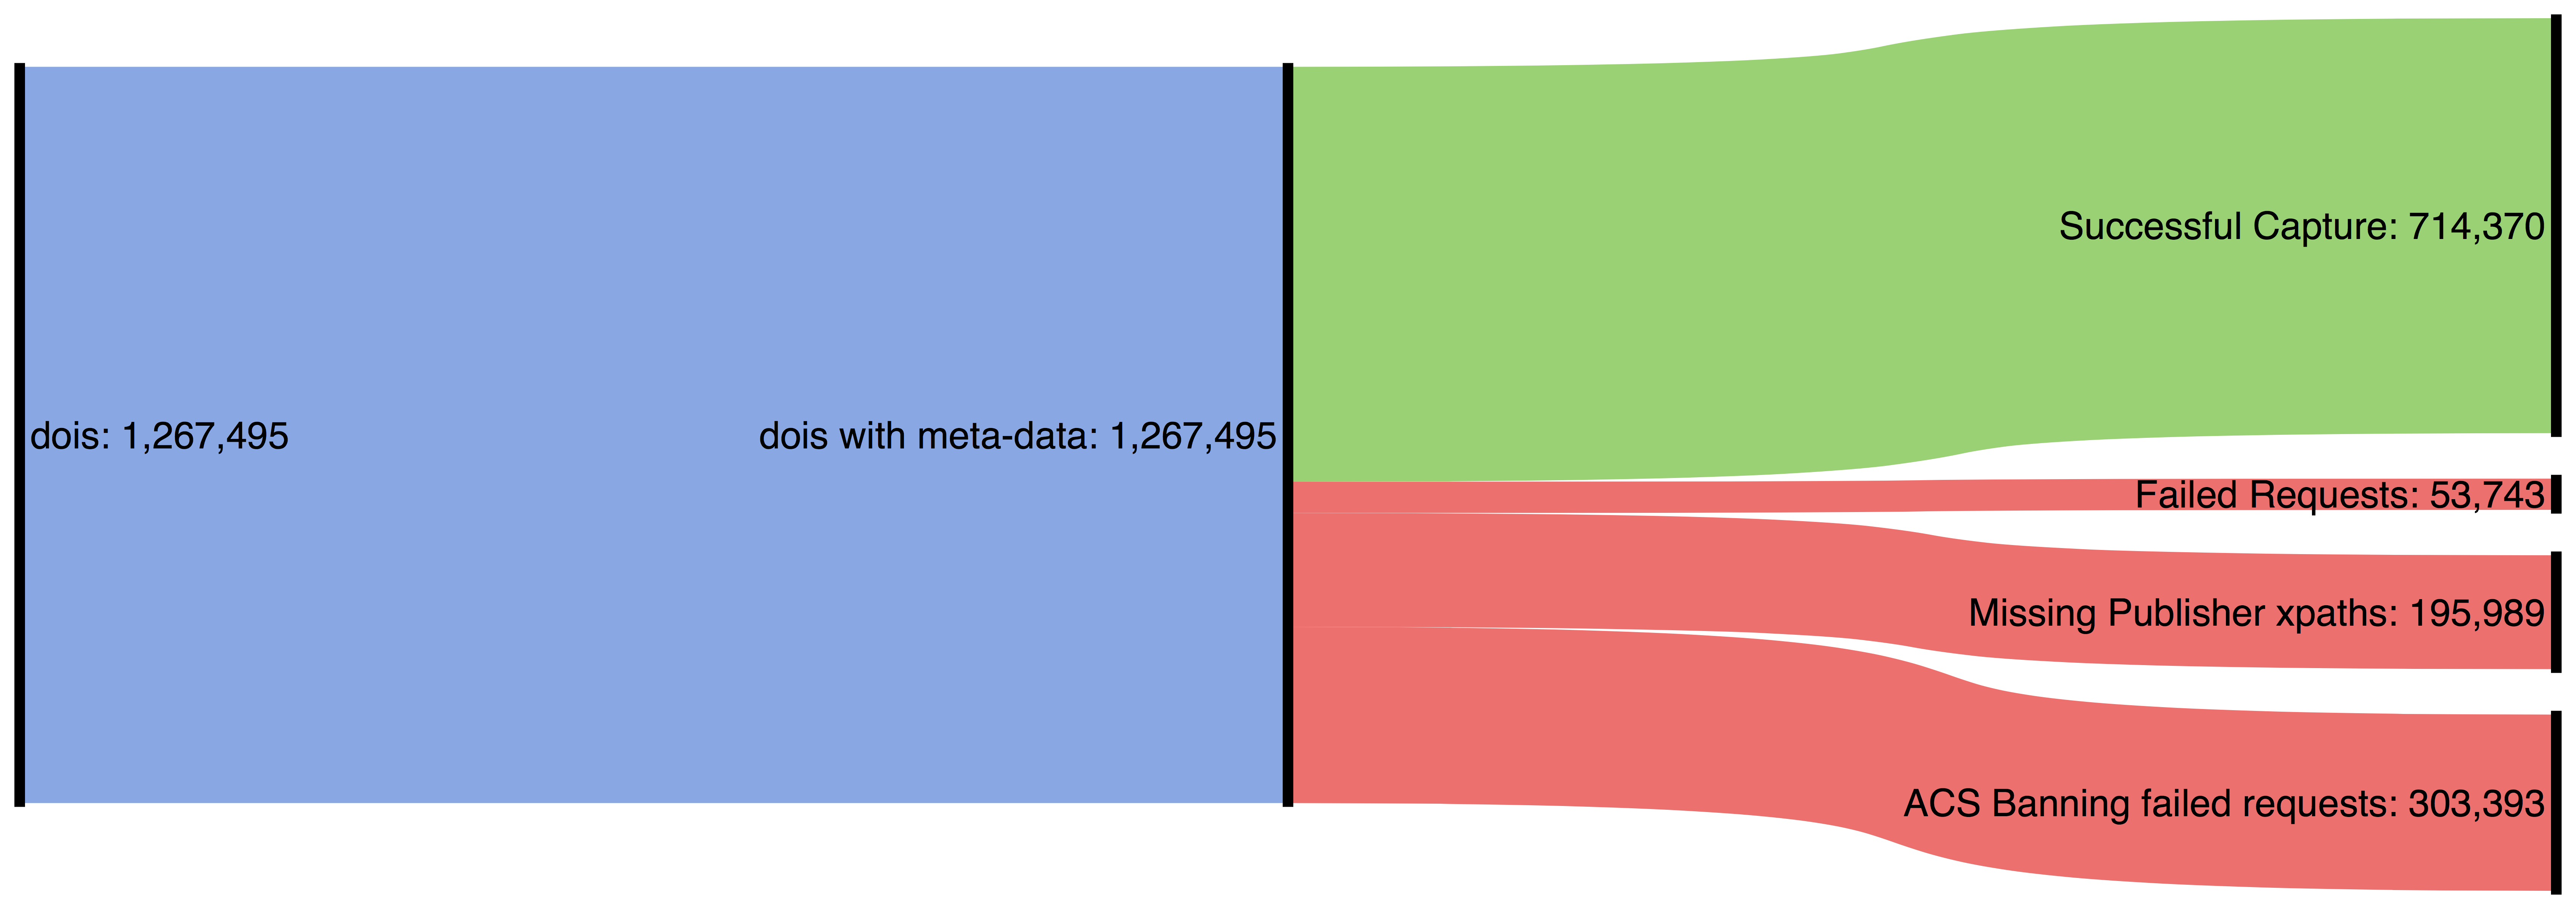
\includegraphics[width=\textwidth]{Data_Acquisition/large_sankey.png}
    \caption[Efficiency of Large Scale Scraping]{The loss processes are coloured red, successfully captured full records in green, and the maximum possible yield in blue.}
     \label{fig:LARGESANK}
\end{figure}

The overall efficiency of the process is 56.4\%, but excluding the acs records lost in the ban, the program's efficiency jumps to 74.0\%, similar to the efficiency of the UK scraping run (\S\ref{sec:UKSCRAPE}). \footnote{Also note that 100\% of dois were converted to dois with metadata. This is because the format of the webpages scraped was consistent for every doi collected.}

The successfully captured 714,370 records were inspected and merged with the UK results. Records were rejected with short titles or abstracts (likely to be addenda, informal articles, retractions etc.) Records were also removed if the majority of the title and abstract were not writen in ascii characters \footnote{ascii is an encoding for English characters a-z, A-Z, some punctuation and 1-9.} (removing majority Japanese and Chinese script). This was done to provide better quality data for training the algorithm described in  \S\ref{chapt:ALGORITHM}. This filtering resulted in a final training database of 464712 articles. This dataset is henceforth referred to as \emph{the training dataset}. The entire database formation process is shown in figure \ref{fig:DATABASES}.
\begin{figure}[H]
    \centering
    \textbf{Summary of Database Preparation}\par\medskip
    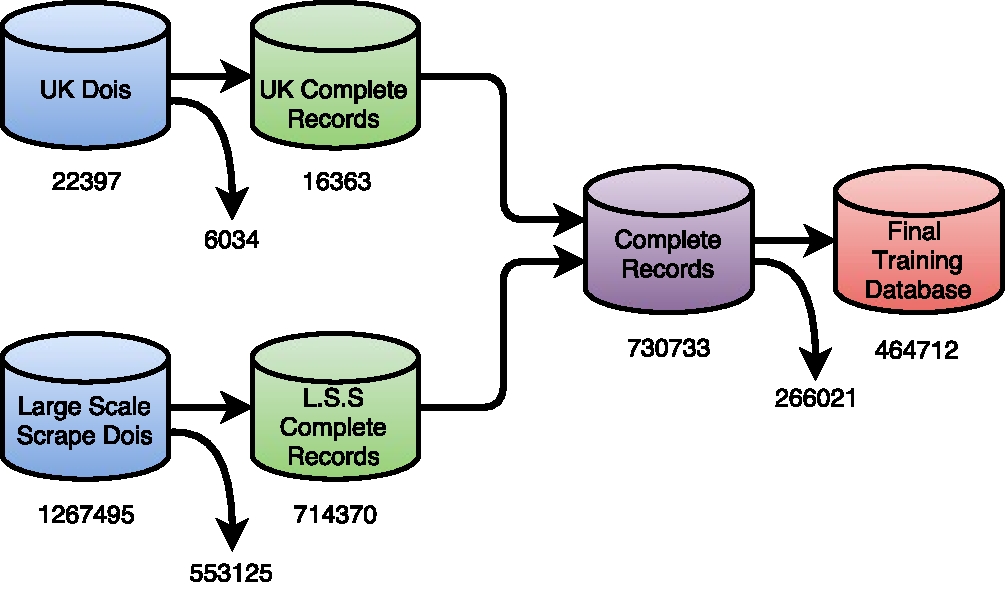
\includegraphics[scale=0.6]{Data_Acquisition/Databases.pdf}
    \caption[Summary of Database Preparation]{Blue databases represent data with dois and metadata. Green databases represent meta-data, dois and abstracts. The purple database is the combined complete records, and the red database is the data deemed suitable for the training algorithm. database sizes and losses are annotated.}
     \label{fig:DATABASES}
\end{figure}


It was instructive to examine these databases and derive some simple statistical results. The following section briefly explores some of these.
\subsubsection{Observations}
\label{sec:CORPUSOBSERVATIONS}
The publisher `market share' can be approximated from examining the database\footnote{Data was taken from `Large Scale Scrape Dois' database, shown in figure \ref{fig:DATABASES}}.
\begin{figure}[H]
    \centering
    \textbf{Publisher Share in Chemistry Literature}\par\medskip
    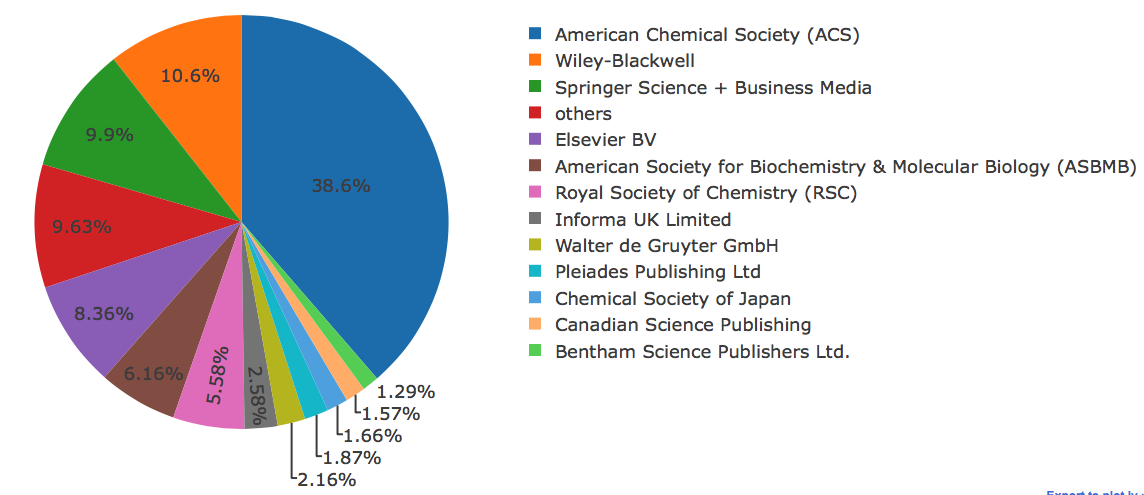
\includegraphics[width=\textwidth]{Data_Acquisition/publishers_pie.png}
    \caption[Publisher Share in Chemistry Literature]{Articles grouped by publisher in the Large Scale Scrape doi database (marked 'Large Scale Scrape Dois' in figure \ref{fig:DATABASES}). Only the top 12 publishers are shown.}
     \label{fig:PUBPI}
\end{figure}
As shown in  shown in figure \ref{fig:PUBPI}, it can be seen that 90\% of all the chemistry literature collected was published by just 12 publishers, the majority from ACS, Wiley-Blackwell, Springer and Elsevier BV. Looking at the UK scraping DOI dataset (Figure \ref{fig:UKPUBPI}), the same large publishers are represented, but the Royal Society of Chemistry has a much larger share. This is to be expected, as the RSC is a UK based body. In the UK, there is a more even distribution between the large publishers. 

\begin{figure}[H]
    \centering
    \textbf{Publisher Share in UK Chemistry Literature}\par\medskip
    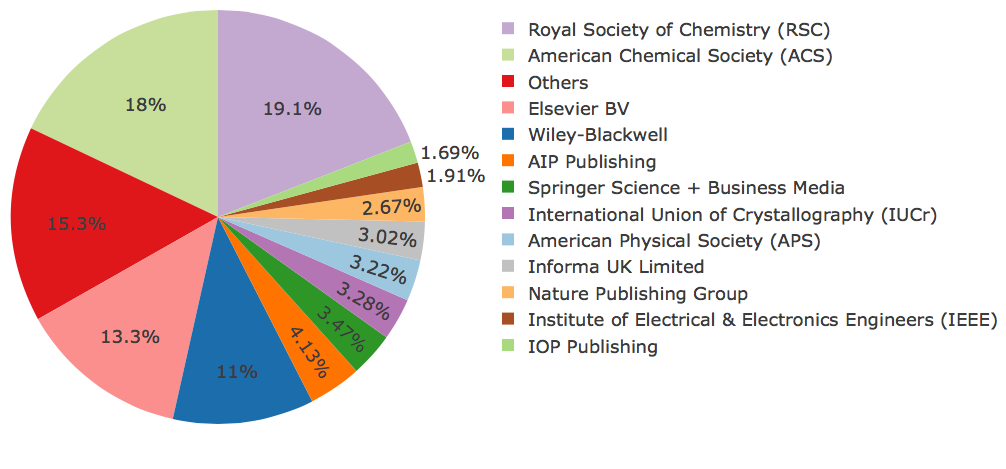
\includegraphics[width=\textwidth]{Data_Acquisition/uk_publishers_pie.png}
    \caption[Publisher Share in UK Chemistry Literature]{Articles grouped by publisher in the UK Doi database published by by each publisher. Only the top 12 publishers are shown.}
     \label{fig:UKPUBPI}
\end{figure}

The corpus of combined titles and abstracts of the complete training database was then examined. The word frequencies across all the data were found to be approximately Zipfian, with a gradient of -1.11\footnote{A Zipfian distribution is a subset of the Pareto distribution, stating that the frequency of a word is proportional to its ranking in the word frequencies table. Ideally, the gradient of a log(frequency) vs log(rank) should be -1.0 \cite{zipf}} See figure \ref{fig:ZIPF}
\begin{figure}[H]
    \centering
    \textbf{Approximate Zipfian Distribution of Collected Corpus}\par\medskip
    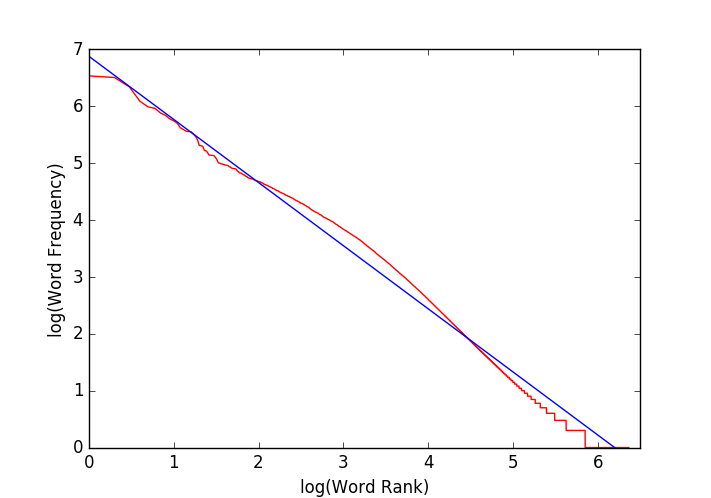
\includegraphics[scale=0.6]{Data_Acquisition/zipf.png}
    \caption[Zipfian Plot of Collected Corpus]{The log Frequency of words vs the log of their position in the rank in the word frequency table in blue. Best fit line in red, gradient = -1.11, intercept 6.3. }
     \label{fig:ZIPF}
\end{figure}
A summary of the corpus statistics are shown below:
\begin{table}[h!]
\caption{Titles and Abstracts in Training Database}
\label{tab:CORPUS STATS}
\begin{center}
\begin{tabular}{||l|c||}
\hline
Total Word Count & 61,296,410\\
Total Unique Words & 2,326,725\\
Total Document Count & 464,712\\
Mode Words per Title &  11\\
Mean Words per Title &  12.2\\
Mode Words per Abstract & 156\\
Mean Words per Abstract & 119.7\\
Mode Sentences per Abstract & 4\\
Mean Sentences per Abstract & 5.4\\
\hline
\end{tabular}
\end{center}
\end{table}

\label{sec:SCRAPEANALYSIS}
